%%%%%%%%%%%%%%%%%%%%%%%%%%%%%%
%%%%%%%% Motivation %%%%%%%%%%
%%%%%%%%%%%%%%%%%%%%%%%%%%%%%%
\chapter{Motivation}

Nowadays machine learning and deep learning have become a distinguished approach for visual
recognition tasks and has achieved great success in this process. However, they seek a large amount of
labeled data to learn. Providing this amount of labeled data not only will bring much effort along but also will occupy a huge size of storage and seek large storage. In
contrast, humans are very good in visual recognition so that, they can learn with one \footnote{This
  is known as one-shot learning in deep learning and represents the scenario when there is one
  instance of each class in training-set to learn.} or few \footnote{This is known as few-shot learning in
  deep learning and represents the scenario when there are just few instances of each class in
  training-set to learn.}
examples. Imagine one kid who can recognize a lion in a picture
after looking a few pictures of lions as an example. We want to simulate and apply this human’s
ability to
the deep learning and make them learn with few examples, with desirable accuracy.
In this bachelor thesis, we concern ourselves with few-shot learning in deep learning. We aim to
learn and train a model when there are few labeled examples obtainable. We approach to generate
artificial examples from a few available labeled examples and enalrge our dataset artificially.
This technique known as data augmentation. These artificial labeled examples aid us to learn better
with more accuracy and prevent overfitting. Data augmentation is our focus in this work to achieve few-shot
learning and prevent overfitting. In this thesis, we will introduce different well-known methods of
data augmentation. The first purpose will be to discover if and how far data augmentation can
improve the learning process and accuracy. The second step will be to compare their accuracy. In
the end, we aim to discover the potential possibility of combining the different methods of data
augmentation to increase accuracy and reduce error-rate and improve the learning process.
We will focus on visual recognition tasks and their classification. Additionally, we will concentrate on the implementation of various methods of data augmentation for convolutional neural networks


%%%%%%%%%%%%%%%%%%%%%%%%%%%%%%
%%%%%%%% Introduction %%%%%%%%
%%%%%%%%%%%%%%%%%%%%%%%%%%%%%%
\chapter{Introduction}

Neural networks can possibly contain multiple non-linear layers and this makes them very expressive models
that can learn very complicated relationships between their inputs and outputs. With even limited
input data, neural networks can discover and learn many relations from the data, however, sometimes the
discovered and learned relations do not exist or just consist of redundant information and
relations. Redudant relation can potentially arise of data-noise or lack of data-generalization. Non
exist relations can potentially emerge from lack of enough data. These phenomena known as
\textit{overffiting} in deep learning. In other words, learning with few labeled examples or noisy
data causes overfitting. Overffiting cause low accuracy and high error-rate. Hence, we approach to propagation of artificial
labeled examples from a few given examples to prevent overfitting and reduce the error rate and increase
the accuracy.

As we mentioned aquiring a huge labeled dataset is expensive and seeks much effort and time. Therefore we aim to generate artificial example from few obtainable labeled examples. In other words, we
augment our data and this strategy is known as data augmentation. There are a few well-known methods for data augmentation. We aim to introduce them in this thesis.  Besides we will implement these
methods to compare their efficiency and capability. These methods are as follow:
\begin{itemize}
  \item \textbf{Label Preserving Transformation} \ref{tit:label-preserving}
  \item \textbf{Elastic Distrotion} \ref{tit:elastic-distrotion}
  \item \textbf{Stroke Warping} \ref{tit:stroke-warping}
  \item \textbf{Bayesian Approach} \ref{tit:bayesian-approach}
  \item \textbf{Manifold Approach} \ref{tit:manifold-approach}
        %\item GANs
\end{itemize}



%%%%%%%%%%%%%%%%%%%%%%%%%%%%%%
%%%%% Data Representation %%%%
%%%%%%%%%%%%%%%%%%%%%%%%%%%%%%
\chapter{Data Representation}
Here should be an Introdution of chapter and introduce the data

\section{MNIST}
The MNIST dataset (Modified National Institute of Standards and Technology) is a large handwritten
digits dataset, provided by Yann Le Cun, derived from NIST Special Database 19 \cite{NIST}.

The MSNIT dataset consists of $60,000$ train- and $10,000$ test-images and each image is grayscale
with $28 \times 28$ pixels. It has $10$ classes that represent $0-9$ digits and data is fairly
splitted between classes \cite{MNIST_data_reference}. MNIST is one of the most popular datasets for
deep learning because of the not too high complexity and compatibility with almost all deep learning
models. Hence many papers attempted to reach a low error-rate on this dataset. One of them manages
to reduce the error-rate on the MNIST by up to $0.23\%$ \cite{MNIST_best_result_reference}. You can
find the information about the dataset at table
\ref{dataset_table} and figure \ref{fig:mnist_dataset_example} shows an example of the dataset.

\begin{figure}
  \centering
  \label{fig:mnist_dataset_example}
  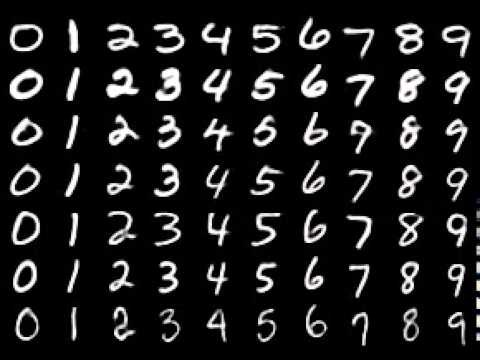
\includegraphics[width=0.5\textwidth]{fig/mnist}
  \caption{7 examples per class of MNIST dataset, merged in one image \cite{MNIST_dataset_example}}
\end{figure}


\section{EMNIST}
blablabla


\section{CIFAR-10}
The CIFAR-10 (Canadian Institute for Advanced Research)
, collected by Alex Krizhevsky, Vinod Nair, and Geoffrey Hinton is a subset from 80 million tiny
images dataset \cite{CIFAR-10_origin_dataset}.

The dataset consists of $60,000$  RGB with $32 \times 32$ pixels images, which are divided to the $50,000$ train and $10,000$ test datasets. As the name makes it clear the CIFAR-10 contains 10 classes ([plane, car, bird, cat, deer, dog, frog, horse, ship, truck]) \cite{CIFAR-10_dataset_reference}.
One of the lowest reported error-rate with a convolutional neural network managed to achieve $2.56\%$ \cite{CIFAR-10_best_result_reference}.  You can
find the information about the dataset at table
\ref{dataset_table} and figure \ref{fig:cifar-10_dataset_example} shows an example of the dataset.

\begin{figure}
  \centering
  \label{fig:cifar-10_dataset_example}
  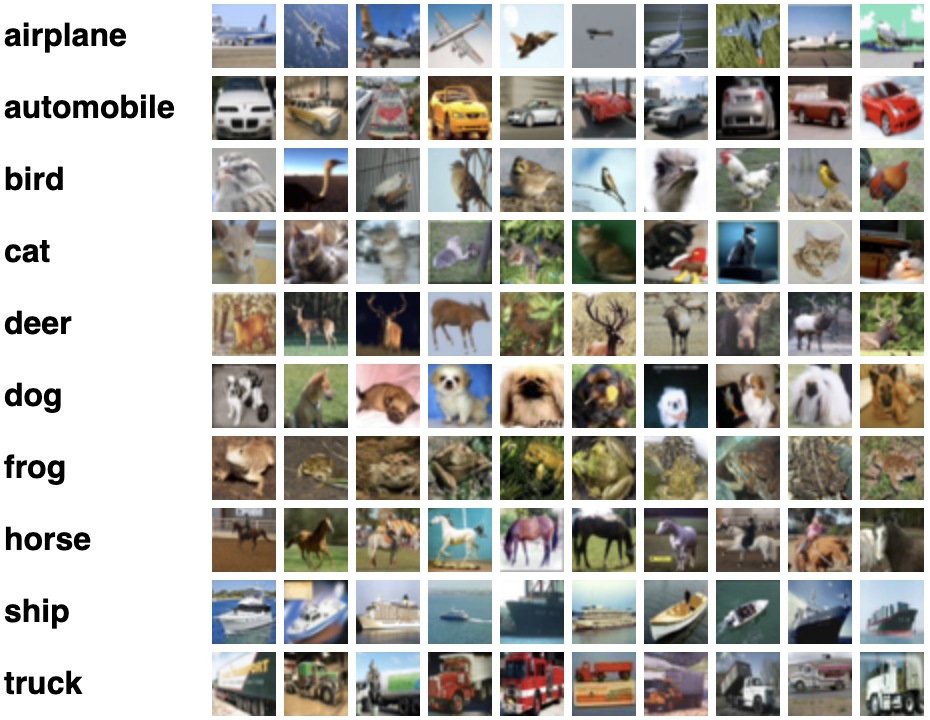
\includegraphics[width=0.5\textwidth]{fig/cifar-10}
  \caption{10 examples per class of CIFAR-10 dataset, merged in one image \cite{CIFAR-10_dataset_reference}}
\end{figure}


\section{CIFAR100}
blablabla


\begin{table}[]
  \label{dataset_table}
  \begin{tabular}{
      l |
      c
      c
      c
      c
      c}
    \hline
    {\textbf{Dataset}}  & \multicolumn{1}{l}{{\textbf{NO. Classes}}} & \multicolumn{1}{l}{{\textbf{NO. Train}}} & \multicolumn{1}{r}{{\textbf{NO. Test}}} & \multicolumn{1}{l}{{\textbf{Size (pixel)}}} & \multicolumn{1}{l}{{\textbf{NO. Channel}}} \\ \hline
    {\textbf{MNIST}}    & 10                                         & 60,000                                   & 10,000                                  & $28\times28$                                & 1 (Grayscale)                              \\
    {\textbf{EMNIST}}   & 26                                         &                                          &                                         &                                             &                                            \\
    {\textbf{CIFAR-10}} & 10                                         & 50,000                                   & 10,000                                  & $28\times28$                                & 3 (RGB)                                    \\
    {\textbf{CIFAR100}} & 100                                        &                                          &                                         &                                             &                                            \\ \hline
  \end{tabular}
  \caption{Structure and organization of the datasets.}
\end{table}


%%%%%%%%%%%%%%%%%%%%%%%%%%%%%%
%%%%% Neural Network %%%%%%%%%
%%%%%%%%%%%%%%%%%%%%%%%%%%%%%%
\chapter{Neural Network}
\section{Introduction}
\section{Convolutional Neural Network}
\section{Overffiting}


%%%%%%%%%%%%%%%%%%%%%%%%%%%%%%
%%%%%%% Data Augmentaion %%%%%
%%%%%%%%%%%%%%%%%%%%%%%%%%%%%%
\chapter{Data Augmentaion}
Here should be Introdution for data augmenation


\section{Label Preserving Transformation}
\label{tit:label-preserving}

One of the most in common method to enlarge the dataset artificially is the label preserving transformation. This method provides the possibility to generate artificial data with
non-heavy computation. The advantage of a very little computation aids us to save storage. In other
words, it wouldn't be required to save the generated data on a storage and the data can always be
enlarged artificially in a short time and with a little computation. As the method's name makes it
clear, this method aims to generate new data from a single data with the same label. We explain the method and its approach for image datasets because as we mentioned our focus is image datasets.

This method consists of generating image translations and horizontal reflectins. Image translations mean, random patches from the original images. The size of the patches are smaller than the
size of the original images. We will extract all pssobile translations (all possible patches which fit in the image) from our image.
These extracted translations (extracted random patches) and their horizontal reflection will be used for training our network. Given a single channel (gray) n$\times$n image and the translation
pathce with size of m$\times$m and $n>m$ then the training dataset will increase by a factor: $$2\times(n-m+1)\times(n-m+1)$$ In the figur \ref{fig:label-preserving-trasformation} is the process of the translations
and reflections of a small image presented.

At test time, the method extracts the patches with the same size. This time the patches will be extracted from 4 corners and center of the original image. The network predicts on these
five patches and their horizontal reflections (10 patches altogether). In the end, the average
of the predictions will be our network's prediction.

\begin{figure}
  \centering
  \label{fig:label-preserving-trasformation}
  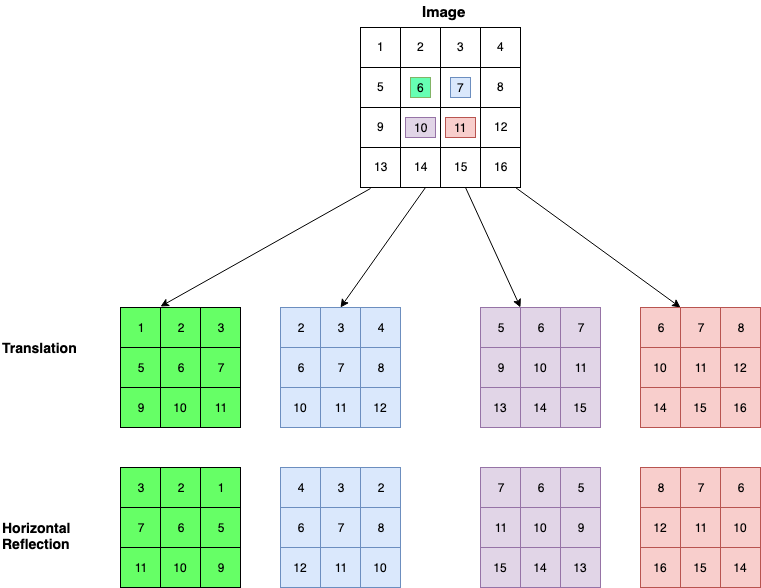
\includegraphics[width=1\textwidth]{fig/label-preserving-transformation}
  \caption{An example of single channel image with size of $4\times4$ with its translations with size of $3\times3$ patches and their horizontal reflections. The numbers determinate the pixels intensity}
\end{figure}


\section{Elastic Distrotion}
\label{tit:elastic-distrotion}
Another well-known method for data augmentation is elastic distortion. This method as the same as label preserving transformation generates artificial data (images) from a single data (image) but with
this difference that this time instead of resizing the image (translation) the pixels inside of the image will be moved and displaced. The intensity of pixels also will be changed with respect to
their new places and their neighbors' intensity and their old places and their origin intensity.

As it cleared elastic distortions concerns itself with a displacement of the pixels and an adjustment of the pixels intensity. This approach is known as interpolation. There are a few schemes like
(nearest neighbor-, bicubic-,  spline- and bilinear interpolation) to reach the goal. Bilinear interpolation is one of the simplest with a desirable result. Hence we use bilinear interpolation. We
will explain the process below.

We will start with pixels displacement. For instance if $\Delta x(x,y)= \alpha x$ and $\Delta y(x,y)= \alpha y$, this means that each pixels will be moved $\alpha x$ in the direction of x-axis and
$\alpha y$ in the direction of y-axis. $\alpha$ would be our scale parameter and since $\alpha$ can be a non-integer value, interpolation is necessary and as we mentioned we use the bilinear
interpolation.  In the next step after pixels displacement, the intensity of the pixels in the new locations should be adjusted concerning the intensity of the neighbors' pixels in the original image
(origin square). Hence bilinear interpolation aids us to reach this target. The bilinear interpolation interpolates the moved pixel horizontally. Then it interpolates the pixel vertically with respect
to yielded values from horizontal interpolations. We will show and summarize the process formally in below.

\begin{definition}{}
  Given $p'$ the pixel which we want to dispalacment it with $\Delta x(x,y)= \alpha x$ and $\Delta y(x,y)= \alpha y$ and $p_{(x,y)}, p_{(x+1,y)}, p_{(x,y-1)}, p_{(x+1,y-1)}$ are the neighbors (on
  origin square) of $p'$ in the new location after displacment and $I(p)$ shows the intensity of pixel $p$. Then the vertical interploation yields:

  $$V_1 = I(p_{(x,y)}) + \big( \Delta x(p', p_{(x,y)}) \times I(p_{(x+1,y)}) \big)$$
  $$V_2 = I(p_{(x,y-1)}) + \big( \Delta x(p', p_{(x,y-1)}) \times I(p_{(x+1,y-1)}) \big)$$

  And then the horizontal interploation yields a new intensity for pixel $p'$ after displacment:
  $$I(p') = V_1 + \big( \Delta y(p', p_{(x,y-1)}) \times V_2) \big)$$
\end{definition}

To reach elastic deformation or elastic distrotion we approach to generate $\Delta x(x,y)= \alpha x$ and $\Delta y(x,y)= \alpha y$ with $\alpha \times rand(-1,+1)$ since $\alpha$ is image-scale parameter
and $rand(-1,+1)$ generate a number between $-1$ and $+1$ with uniform distribution. After all, the
fields $\Delta x$ and $\Delta y$ are convolved with a Gaussian filter with standard deviation of
$\sigma$. The values of $\sigma$ and $\alpha$ depends on the image size and the image entropy. This process will generate elastic deformed image from orginal image which called elastic distrotion.


\section{Stroke Warping}
\label{tit:stroke-warping}
This method as same as previously introduced methods uses predetermined families of transformations.
In other words, we enlarge our dataset artificially with the aid of well-known classical computer
vision transformations. This method notwithstanding of non-heavy complexity accomplished desirable
results even on medical purposes \cite{stroke_tumor}. The ideas of this Methode raised from Tangent
Dist and Tangent Prop \cite{stroke_idea_1992} and \cite{stroke_idea_1993} works. 

In this method, we perform small changes in images to augment our data.  That means we augment our
images with skewing, rotating and shearing them \cite{storke_warping_1997_source}. As same as the
label preserving transformation and elastic distortion the augmentation will be started before the
training phase and the training will be performed on enlarged data. In figure
\ref{fig:stroke_warping_transforamtions} represents each mentioned translation to make them visually
understandable.

\begin{figure}
  \centering
  \label{fig:stroke_warping_transforamtions}
  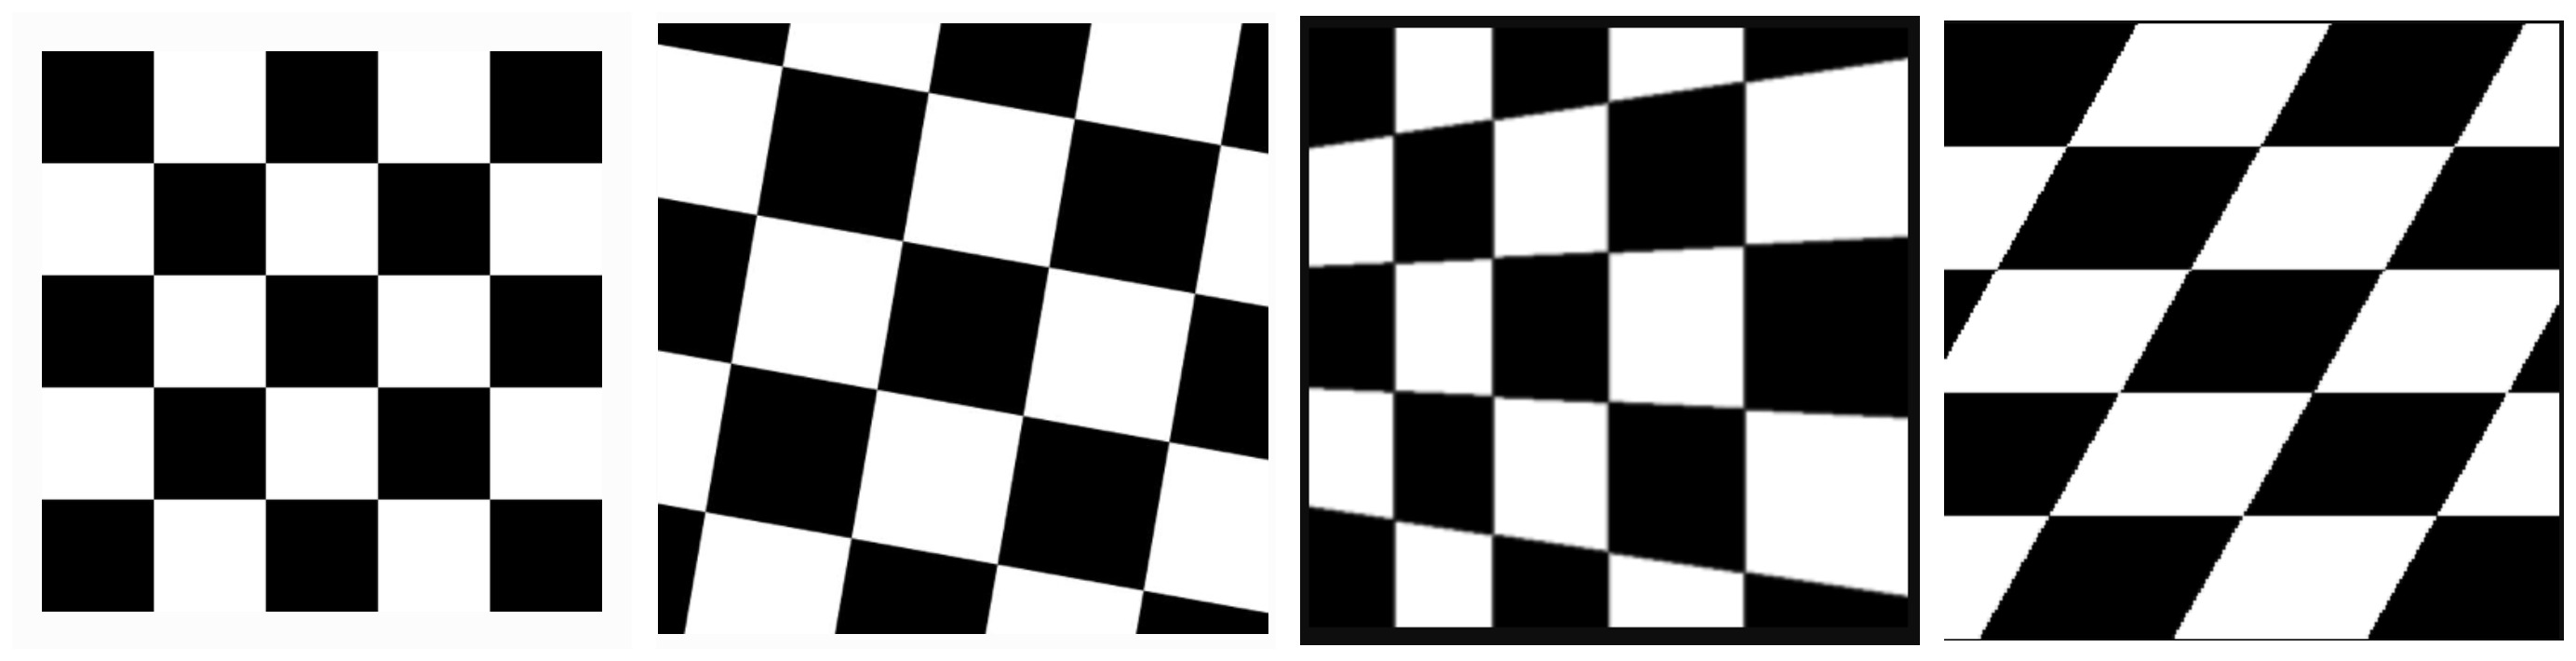
\includegraphics[width=1\textwidth]{fig/stroke_warping_transforamtions}
  \caption{An exmaple of rotation, skew, shear, and scale translations for stroke warping respectively from left to right. The first image from left is the orginal image \cite{TODO-Augmentaion}}
\end{figure}


\section{Bayesian Approach}
\label{tit:bayesian-approach}
As you may until now realized, all introduced classes of techniques in this work for data augmentation were pre-defined families of statistical transformations. In other words, we generated synthetic images with computer vision techniques statistically before the training phase and we didn't change our augmented data until the end of the learning. In fact, the basic idea of each of them is known as “poor man’s” data augmentation (PMDA) \cite{poor_man_data_augmentation}. The point is if neural networks, in general, can learn such complex relations and patterns in images, therefore they should be able to learn latent variables to improve data augmentation dynamically. Put the matter another way, in this method, we focus not only on the classification task and learning patterns of images but also on learning how to improve our image augmentation dynamically and iteratively during the training and classification. 


\section{Manifold Approach}
\label{tit:manifold-approach}

\chapter{Comprehensive Comparison}

\chapter{Mthodes Combination and new method}